\begin{quote}
\textit{``Where are you?'' Hiro says.
\\
\\
``In Reality or the Metaverse?''
\\
\\
``Both.''}
\end{quote}
\hfill \textit{Snow Crash, Neal Stephenson}
\\
\\
\\

%=========================================================================================================
%=========================================================================================================

% 'Position' section from experimental plan document

%\section{Introduction}
This research centres around the design, development \& evaluation of a hardware \& software platform which allows its user to observe \& move around their Real World (RW) environment whilst wearing a wide field of view (FOV), stereoscopic 3D, Head Mounted Display (HMD) which allows them to alternatively view an immersive Virtual Reality (VR) environment from the equivalent vantage point. This is achieved by combining a head-tracked HMD, webcams, an indoor positioning system (IPS) \& a 3D game engine, into a mobile \textit{cross reality} (XR) interface.

One of the distinguishing features of XR is that, by linking real \& virtual environments more closely, it mitigates the `vacancy problem': \textit{``the noticeable \& profound absence of a person from one world, either real or virtual, while they are participating in the other''}, which arises \textit{``because people do not currently have the means to be in more than one place (reality) at a time''}~\cite{Lifton2007a}.

Previous XR research approached the vacancy problem by integrating sensor/actuator networks into the environments, such that actions in one could manifest in the other, however direct visual engagement with the virtual environment was only possible from static interfaces at pre-determined locations within the real environment~\cite{Lifton2007a, Dublon2011}. The platform discussed in this document addresses this shortcoming by providing a mobile interface for visual engagement with both environments of a XR system, allowing the user to transition between viewing their real environment \& a virtual environment at any time while maintaining the freedom to move around them, multiplexing visual stimuli from their real surroundings \& from a parallel, virtual `mirror world'~\cite{Gelernter1993}.

%=========================================================================================================
%=========================================================================================================

\section{Defining Alternate Realities}
A fundamental imperative for the remainder of this review is a well defined set of criteria for classifying and differentiating between different types of alternate reality. The terms \textit{mixed reality}, \textit{augmented reality} and to a lesser extent \textit{augmented virtuality} are all now relatively common in the literature, however they have too often been used in conflicting manners, or assigned vague definitions with uncertain boundaries separating them from each other. Furthermore the less well established terms \textit{cross reality} and \textit{X reality} (different names for the same concept) also need classifying according to the same system.

%=========================================================================================================
%=========================================================================================================

% From.... original lit review?

Research on alternate realities has been extensive, with the theme being explored for purposes as diverse as education~\cite{Warburton2009} and new forms of data visualisation~\cite{Coleman2009} to medical~\cite{TenEyck2011} and military training~\cite{Qiu2009}. Traditionally access to implementations of alternate realities was limited by the availability and high monetary cost of the specialised hardware and software that was required to create virtual environments and computerised superimpositions~\cite{Druck2006}. However more recently the cost and availability of this hardware and software has reduced and increased respectively to the point at which we find ourselves today where alternate realities can be, and in fact frequently are, experienced by many with the equipment they already have available to them with no special considerations~\cite{Sevan2008}.

Hardware capable of synthesising the graphically complex three-dimensional environments that alternate realities often present has reduced in cost to the point that it is no longer considered specialist equipment, owned only by those expressing an explicit interest in the subject, and is now commonplace in `average' consumer electronics devices, be they traditional desktop and laptop computers, games consoles, or portable devices such as mobile phones and tablets. Combined with the continued adoption of high-speed Internet connectivity~\cite{Cisco2011} the potential of multi-user virtual environments is already being realised, both for traditional competitive gaming through platforms such as World of Warcraft, but also for non-competitive purposes that focus more on community, creation and commerce with `virtual world' platforms such as Second Life~\cite{Sevan2008}.

Furthermore, progress toward ubiquity of sensing and actuating infrastructure in our everyday lives continues at an accelerated rate~\cite{Bose2009, Baronti2007}. Such systems are now commonplace in new buildings and also in consumer electronics, both portable devices such as mobile phones and tablets as well as home entertainment products such as games consoles. The result is that the amount of information that we can access about the physical and environmental state of a particular location at any given time is greater than ever.

The combination of these factors means that we are approaching the required dissemination of technology and public knowledge and understanding for virtual environments and integration with sensor/actuator infrastructure to begin making a larger impact on society and ultimately to be used by on a scale and in a manner similar to how the World Wide Web already is today. It is no longer preposterous to imagine a near future where a `Metaverse' reminiscent of that in Neal Stephenson's cyberpunk novel \textit{Snow Crash}, presenting an extension of the Web in the form of a three-dimensional virtual environment, has become a reality adopted by the majority of current Web users rather than remaining a vision of academics and cyberpunk fiction aficionados.

However although there are numerous examples of virtual environments, particularly those for competitive gaming, gaining substantial popularity~\cite{Sevan2008} and augmented reality and augmented virtuality products are no longer restrained to the research lab, this review has found very little research into simultaneous presence in \textit{complete} real and virtual environments. The term \textit{complete} is used to emphasise that the discussion here is about real and virtual environments that are both complete unto themselves and which can thus be explored and interacted with in isolation from the other, in addition to being explored simultaneously. This is a different concept to augmented reality and augmented virtuality systems, where the augmentations are usually near meaningless when separated from the context bestowed upon them by the underlying environment that they are augmented upon.

The \textit{cross reality} paradigm represents the most promising foray into investigation of this concept, as such a system is established through the combination of two complete environments, a real environment and a virtual environment that is based upon and mimics this real environment, which are bestowed with the abilities of mutual reflectance and influence through the use of sensor/actuator infrastructure (see section \ref{sec:cross_reality} for full discussion). Physical and environmental changes in the state of the real environment are captured by sensors and these data used to update the state of the virtual environment, whilst simultaneously changes in the state of the virtual environment manifest into the real environment via actuators. Users are free to explore and interact with either environment in relative isolation from the other, even if their interactions in one trigger changes in the other, however simultaneous interaction and exploration with both environments has largely remained without systematic investigation.

This is largely because users exploring and interacting with the real environment do not have a convenient manner of also exploring and directly interacting with the virtual environment, as such interaction usually relies upon the use of software run on a desktop or laptop computer which is not conducive to mobile use. Using a laptop computer whilst walking around is far from convenient and using a desktop computer obviously limits the user's interaction with the real environment to that immediately around the location of the  computer and results in a disjoint relationship between their physical position in the real environment and the location of their avatar in the virtual environment when they navigate their avatar away from the respective position of their computer. This situation has been called `the vacancy problem'; an apparent vacancy from one environment whilst engrossed in the other (see section \ref{subsec:dual_reality_:_an_emerging_medium} for full discussion).

Interested in the promise of simultaneous presence in complete real and virtual environments, particularly those that are able to mutually affect each other via sensor/actuator infrastructure and the cross reality paradigm, this literature review investigates how academic studies have treated such themes. The conclusion of this investigation is that the theme of simultaneous presence in real and virtual environments is still discussed only marginally in the scholarly literature and that this situation warrants attention as the benefits proposed by such interactions between real and virtual environments are extremely promising.

%=========================================================================================================
%=========================================================================================================

\subsection{Milgram \& Kishino's Reality Continua}
Paul Milgram, Herman Colquhon and Fumio Kishino addressed this issue in detail and can in fact be accredited with introducing the terms \textit{augmented virtuality} and \textit{mixed reality} to the literature in the first instance, prompted by their identification of the need for more encompassing terms to supplement the existing definitions of \textit{augmented reality}~\cite{Milgram1994, Milgram1999}. Their discussion at times takes on a hint of the philosophical, as it rightly discusses what exactly it is that we mean by `real' and `virtual' and whether it is in fact reality or virtuality which is being augmented. However despite these thorough and well-reasoned definitions being published originally in 1994, much of the subsequent literature studied for this review has adopted conflicting, or at least confusing and misleading, definitions.

One of the overbearing concepts that Milgram et al. introduced is that whilst both purely real and purely virtual environments do exist they should not be considered discrete alternatives but rather poles lying at opposite ends of a linear scale called the \textit{Reality-Virtuality continuum}. The location of an environment along this continuum coincides with its location along a parallel \textit{Extent of World Knowledge continuum} where `world knowledge' refers to the amount of quantitative information that is associated with the content being presented, or in other words how much of the environment is being `modelled' by a computer. These continua are included as figure \ref{reality_virtuality_extent_of_world_knowledge_continuum}.

\begin{figure}[h]
\centering

\includegraphics[width=\textwidth]{virtuality_continuum_extent_of_world_knowledge_continuum.png}
\caption{\textit{Reality-Virtuality continuum} (top), parallel with \textit{Extent of World Knowledge continuum} (bottom).}
\label{reality_virtuality_extent_of_world_knowledge_continuum}
\end{figure}

With a purely virtual environment, the entire viewport must necessarily be computer modelled in order to be rendered and as such there is complete quantitative information about all objects and between all objects being presented. At the opposite end of the spectrum with a completely real environment where none of the viewport is computer modelled there is no quantitative information associated with the content being displayed. At any point between the extremes the environment consists of a mixture of some modelled and some non-modelled content; with the computer associating quantitative information to, and between, the virtual objects, but not to the real objects or between the virtual and real objects.

Carrying the continuum concept further, Milgram et al. illustrate their understanding of the existing term \textit{augmented reality} and also introduce two related new terms; \textit{augmented virtuality} and \textit{mixed reality}. In this fashion, \textit{mixed reality} is used to describe any environment that is not completely real or completely virtual; that is, it encompasses all positions on the continuum between the extremes. \textit{Augmented reality} is used to describe a real environment upon which virtual objects are overlain and \textit{augmented virtuality} is used to describe a virtual environment upon which objects sampled from the real world (such as video feeds) are overlain. It is also shown here that \textit{mixed reality} encompasses both \textit{augmented reality} and \textit{augmented virtuality}.

One obvious question raised from studying this figure is at what point toward the centre of the continuum an environment changes from being \textit{augmented reality} into \textit{augmented virtuality} or vice-versa. The answer lies with consideration of the quantitative knowledge associated with the objects that comprise the viewport.

For example, if one were to take a viewport depicting a purely real environment and then incrementally add more and more virtual objects, the environment's classification would progress rightward along the continuum. Eventually the entire viewport would be obscured by virtual objects and the obvious conclusion would be to classify the environment as being purely virtual. However this would only be true if there was complete quantitative information associated with, and between, all of the virtual objects within the real 3D space of the viewport, which is unlikely to be the case.

Likewise if one were to take a viewport depicting a purely virtual environment and incrementally replace the entire viewport with sampled real objects we could not classify the resultant environment as purely real as there would be associated quantitative knowledge with and between the sampled objects, meaning that the environment isn't completely unmodelled and thus can't be classified as purely real.


Thus, Milgram et al. conclude, it is not necessarily true that an environment is purely virtual simply because all of the visible objects are computer modelled, nor is it necessarily true that an environment is purely real simply because all of the visible objects are sampled from the real world.


\subsection{Waterworth \& Waterworth's Three Dimensions of Virtual Experience}
\newcommand{\presencefootnote}{\footnote{\textbf{Presence} in this context is defined as a state of heightened perceptual processing of environmental stimuli (\textit{``a psychological focus on direct perceptual processing''}~\cite{Waterworth2001}) accompanied by lessened conceptual reasoning, whether these environmental stimuli originate from a real environment, a virtual environment, a mixed reality environment, or even from multiple discrete environments.}}

\newcommand{\absencefootnote}{\footnote{\textbf{Absence} is defined as \textit{``a psychological focus on \ldots conceptual processing''}~\cite{Waterworth2001}.}}

\textbf{Haven't actually mentioned anything about presence in the review so far, have we?}

The virtuality continuum is here considered to be analogous to the \textit{locus of attention} axis of Waterworth \& Waterworth's \textit{three dimensions of virtual experience} model~\cite{Waterworth2001}; the combination of these models is shown by figure \ref{focus-locus-sensus-with-virtuality-continuum}. In this model, locus of attention represents the environment where the stimuli that the user is perceiving originate from; focus of attention represents the balance between conceptual/abstract reasoning \& perceptual/concrete processing, where complex conceptual reasoning results in little attention being paid to processing environmental percepts (whether originating from real or virtual stimuli) thus reducing presence\presencefootnote{} in that environment toward its antithesis $-$ absence\absencefootnote{}; and sensus of attention represents the level of conscious arousal (or `wakefulness'~\cite{Laureys2009}) of the user, whether directed toward percepts originating from real stimuli, virtual stimuli, a mix, or not directed toward any percepts in the case of completely `absent' conceptual reasoning.

\begin{figure}[h]
	\begin{center}
		
\includegraphics[width=0.685\textwidth]{focus-locus-sensus-with-virtuality-continuum.png}
		\caption{The combined virtuality continuum/three dimensions of virtual experience model.}
		\label{focus-locus-sensus-with-virtuality-continuum}
	\end{center}	
\end{figure}

%The Sensus Dimension - the importance of being awake in class
%"Even as we sleep dreamlessly..." (example of being 'unconscious' in this regard)

%fourth axis is alterity, between hermeneutics \& embodiment

%=========================================================================================================

\subsection{Reality Matrix}
\label{subsec:reality_matrix}
Another useful method of illustrating the relationships between the different categories of alternate realities was put forward by Roy Want in his introductory article for a 2009 issue of IEEE Pervasive Computing dedicated to the \textit{cross reality} paradigm~\cite{Want2009}. Here he presented a 2x2 matrix categorising the different terms according to whether the experience and overlay data are real or virtual (see figure \ref{original_virtuality_matrix.png}).

\begin{figure}[h]
\centering
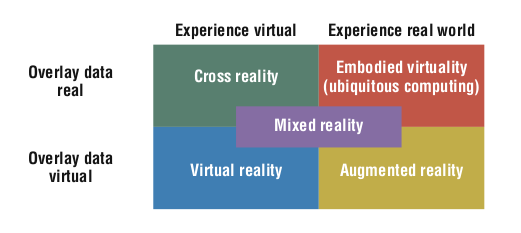
\includegraphics[width=0.8\textwidth]{original_virtuality_matrix.png}
\caption{Want's original virtuality matrix.}
\label{original_virtuality_matrix.png}
\end{figure}

Whilst this is a useful representation, some of the definitions and criteria depicted do not match with those of Milgram et al. or even with those of other authors in the same issue of IEEE Pervasive Computing, let alone other publications concerning alternate realities. Thus this review presents a modified version of Want's matrix, that is better in fitting with the consensual definitions built from reviewing the literature on alternate realities, as figure \ref{modified_virtuality_matrix.png}.

\begin{figure}[h]
\centering
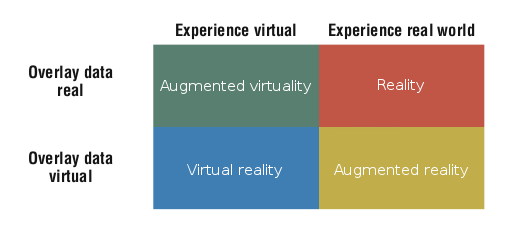
\includegraphics[width=0.8\textwidth]{modified_virtuality_matrix.png}
\caption{Want's virtuality matrix after modification by this review; note removal of \textit{mixed reality}, \textit{cross reality} and \textit{embodied virtuality} and addition of \textit{reality} and \textit{augmented virtuality}.}
\label{modified_virtuality_matrix.png}
\end{figure}

Where Want has \textit{cross reality} occupying the upper left quadrant at the congruence of `experience virtual' and `overlay data real' this review instead places \textit{augmented virtuality}. Referring to Milgram's continuum `experience virtual' relates to a position somewhere on the right half, while `overlay data real' relates to presentation over this virtual environment of sampled real world data resulting in a partially modelled environment, leaving us in the area of the continuum occupied by \textit{augmented virtuality}.

Want's matrix also features the term \textit{embodied virtuality} in the upper right quadrant, at the congruence of `experience real world' and `overlay data real'. Want explains that this is an alternative term for \textit{ubiquitous computing} which is \textit{``essentially the opposite of VR''}; this review instead reasons that the opposite of \textit{virtual reality} is simply \textit{reality} and that \textit{ubiquitous computing} does not constitute an alternate reality but simply a different model of human-computer interaction that can be implemented in either \textit{reality} or \textit{augmented reality}, depending upon how the computing infrastructure presents information to users.

A \textit{ubiquitous computing} system is necessarily a real environment, as it is by definition the integration and dissemination of computational infrastructure into our real surrounds~\cite{York2004}. However whether this real environment is augmented by virtual objects is not restricted by the concept. Thus \textit{ubiquitous computing} can exist in an environment that is either on the left extreme of the continuum, where no virtual objects are employed and the environment remains completely unmodelled, or somewhere to the right of the left extreme in the region of \textit{augmented reality}, where virtual objects are employed and the environment is partially modelled.

This line of reasoning is supported by an almost complete lack of further mention of \textit{ubiquitous computing} elsewhere in the literature about alternate realities studied for this review. Furthermore the term \textit{embodied virtuality} is not used by any other author in the studied literature.

Finally this review has removed the central \textit{mixed reality} section from Want's original matrix, as its position could be misleading. As the boundaries formed between the categories by the different colours could be construed as meaning that there are discrete boundaries between the different categories, rather than a linear scale as depicted by Milgram's continuum, the reader could be led to believe that a purely \textit{virtual reality} or a purely \textit{embodied virtuality} environment can be considered \textit{mixed reality}, which is incorrect. If one wishes to picture the position of \textit{mixed reality} in relation to the modified matrix, it would cover the same area as enclosed by the union of \textit{augmented virtuality} and \textit{augmented reality}.

\subsection{More Reality Continua}
As one of the most prominent academics in the development of the cross reality paradigm (see section \ref{sec:cross_reality}) it is also worth comparing Joshua Lifton's definitions for the different categories of alternate realities and the relationships between them~\cite{Lifton2007a} in the current context.

Lifton's definitions, or more accurately his relationships between, the terms \textit{reality}, \textit{augmented reality}, \textit{mixed reality} and \textit{virtual reality} do not perfectly match the consensus that this review has observed. Lifton defines the terms individually in agreement with the consensus, however doesn't proffer the conclusion that mixed reality is a broad term that includes augmented reality. He also doesn't mention augmented virtuality, even though the Dual Reality Lab project (see section \ref{subsec:mit_shadow_lab}) does implement it. Finally his diagram that alludes to Milgram's continua and is included as figure \ref{original_lifton_axis.png}, situates mixed reality at an incorrect position, implying that Lifton's definition of mixed reality is of a discrete state to that of augmented reality, even though his textual definition of mixed reality hints that it logically encompasses augmented reality. This review presents a modified version of Lifton's diagram to illustrate these differences as figure \ref{modified_lifton_axis.png}.

Lifton does however explain that while such a taxonomy can be successfully applied to most alternate reality efforts, it does not well address the concept of cross reality where there are two complete realities, one real and one virtual.

\begin{figure}[h]
\centering
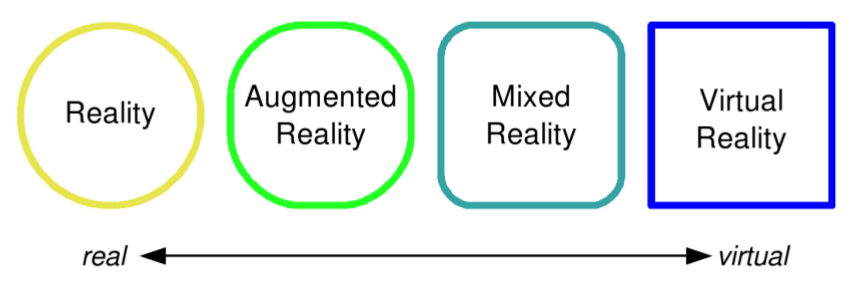
\includegraphics[width=\textwidth]{original_lifton_axis.png}
\caption{The \textit{``virtual worlds taxonomy as viewed on the real-virtual axis''} presented by Lifton.}
\label{original_lifton_axis.png}
\end{figure}

\begin{figure}[h]
\centering
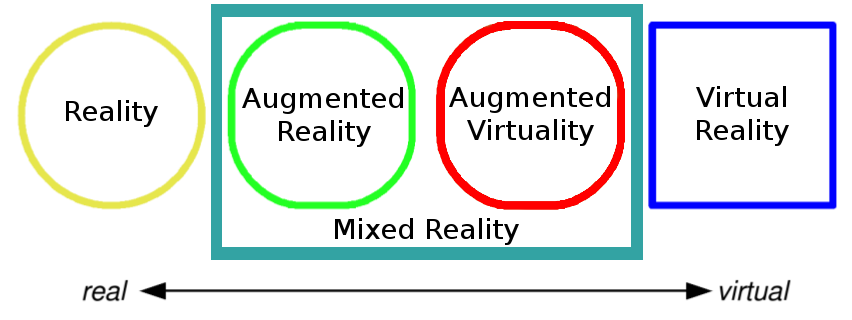
\includegraphics[width=\textwidth]{modified_lifton_axis.png}
\caption{Lifton's taxonomy as modified by this review.}
\label{modified_lifton_axis.png}
\end{figure}

%=========================================================================================================

\section{Adopted Definitions of Alternate Realities}
\label{sec:definitions_of_alternate_realities}
This review has discovered differing (and in some cases conflicting) definitions for the different categories of alternate realities and for the criteria for differentiating between them. What follows in this section represents the definitions and differentiating criteria that this review has adopted after concluding them the most widely accepted and well reasoned.

\subsection{Reality}
Occupying the left extreme of Milgram's continuum and the upper right quadrant of the modified Want matrix, \textit{reality} refers to an environment that is entirely unmodelled, with the viewport containing no virtual objects and no computer-based quantitative information is associated with any of the (necessarily real) objects. In fact, there may be no computer infrastructure involved in the situation whatsoever. This is the situation that we are most familiar with, as it is where the vast majority of us spend the vast majority of our time.

\subsection{Virtual Reality}
The polar opposite to \textit{reality}, a \textit{virtual reality} environment occupies the right extreme of Milgram's continuum and the lower left quadrant of the modified Want matrix. A \textit{virtual reality} environment consists solely of virtual objects, with computer-based quantitative information associated with all of them and between all of them, creating a completely synthetic world entirely discrete and separate from the real world; a new world that exists solely within the data structures of a computer.%cite Milgram and Want

Traditional definitions of \textit{virtual reality} require the environment to be completely immersing; that is, when involved with such an environment the user is completely unaware of the real environment that surrounds their real bodies, often making use of Head Mounted Displays (HMD) and head \&/or body tracking techniques to improve the sense of immersion by removing the need to interact with interfaces logically anchored to the real world such as keyboards, mice and joysticks~\cite{Druck2006}.

However this review believes that taking the concept to a lesser extreme, the virtual environments presented by video games such as World of Warcraft can be construed as \textit{rudimentary} implementations of virtual reality; they are completely modelled environments that exist entirely separate to the real world, however interaction is not completely immersing due to the use of 2D monitors and traditional interface devices, largely due to the lack of common ownership of HMDs and advanced body tracking systems.

\subsection{Mixed Reality}
Occupying any position between the extremes on Milgram's continuum, the term \textit{mixed reality} refers to a broad range of environments that arise from the merging of real and virtual environments to some extent such that the result is neither entirely real nor entirely synthetic, where real and virtual objects co-exist. As alluded to previously, under this definition both \textit{augmented reality} and \textit{augmented virtuality} are included under the broader classification of \textit{mixed reality}.

This is one definition where Want is lacking, claiming \textit{mixed reality} to be \textit{``some combination of the others''} where `others' refers to all of \textit{virtual reality}, \textit{augmented reality}, \textit{embodied virtuality} and \textit{cross reality}. This review disregards this definition as it relies upon Want's previously refuted definition of \textit{embodied virtuality} being the polar opposite of \textit{virtual reality} and because it also depends upon Want's definition of \textit{cross reality} which this review will also go on to refute.

\subsection{Augmented Reality}
An \textit{augmented reality} environment occupies a position within the `left half' of Milgram's continuum, the lower right quadrant of the modified Want matrix and within the broader classification of \textit{mixed reality}. Thus an \textit{augmented reality} environment comprises a real environment that has had virtual objects added to or overlain upon it; a common approach for achieving this addition/overlay is superimposing virtual objects over a direct or indirect view of the real environment using Head Mounted Displays \&/or cameras~\cite{Krevelen2010}.

A commercial example of \textit{augmented reality} is the Layar browser for mobile phones, which overlays various forms of data onto the view captured by a phone's camera after determining its location and orientation using GPS, accelerometer and magnetometer readings~\cite{eishita:layar}

%~\cite{Milgram1999}

\subsection{Augmented Virtuality}
Logically opposite to \textit{augmented reality}, an \textit{augmented virtuality} environment occupies a position within the `right half' of Milgram's continuum, the upper left quadrant of the modified Want matrix and again lies within the broader classification of \textit{mixed reality}. Thus an \textit{augmented virtuality} environment comprises a virtual environment, akin to \textit{virtual reality}, upon which sampled real objects are overlain, perhaps through the use of cameras~\cite{caballero:behand}.

A simple commercial example of augmented virtuality is the EyeToy accessory and associated software for Sony's Playstation 2 games console (and later the Playstation Eye for the Playstation 3), a digital camera that captures images of players and their surroundings and integrates them into the gaming experience presented on the screen.

%=========================================================================================================
%=========================================================================================================

\section{Cross Reality}

\label{sec:cross_reality}
The discussion of the literature pertaining to the \textit{cross reality} paradigm warrants its own section of this review, as it is not only one of the youngest categories included under the umbrella term \textit{alternate reality} but also the closest existing concept to lend to the simultaneous exploration of real and virtual environments.

\subsection{Overview of Cross Reality}
Cross reality is the ubiquitous mixed reality situation that arises from the fusion of real-world sensor/actuator infrastructure with virtual environments, such that augmented reality and augmented virtuality manifest simultaneously and facilitate synchronous multi-directional exchange of media and control information between real and virtual environments. Sensors collect and tunnel dense real-world data into virtual environments where they are interpreted and displayed to dispersed users, whilst interaction of virtual participants simultaneously incarnates into the real world through a plenitude of diverse displays and actuators~\cite{Paradiso2009}.

The principle features that distinguish cross reality from other alternate realities that this review has thus far covered are;
\begin{enumerate}
	\item a shift from single- to bi-directional information flow between real and virtual environments~\cite{kim:practical}
	\item that both environments are complete unto themselves (but are enriched by their ability to mutually reflect, influence and merge into one another).~\cite{lifton:merging}
\end{enumerate}

\textbf{This thesis presents systems that focus on the second aspect above \& extends it by permitting both environments to be experienced at any time \& position.}

\subsection{MIT Media Lab Responsive Environments Group}
\label{subsec:responsive_environments_at_mit_media_lab}
The Responsive Environments Group at MIT's Media Lab, under the direction of Joseph Paradiso, deserve the accolade for the inaugural work in establishing cross reality as a field of research. In their own words, the group \textit{``explores how sensor networks augment and mediate human experience, interaction and perception''}~\cite{ResponsiveEnvironmentsGroup} and since 1995 they have produced prolific research in the domain of sensor architecture and wireless sensor clusters~\cite{Paradiso1996, Rowe1999, Burke1996, Paradiso1997, Knaian2000, Teegarden2001, A2007, Ma2002, Bamberg2008, Laibowitz2005, LaPenta2007} and perceptive spaces~\cite{Lifton2001, Paradiso1997a, Paradiso2000, Richardson2004}, establishing a prime research environment, both in terms of experience and available technologies, for a concept such as cross reality to emerge.

The path to cross reality began with the `Plug' project that created a sensor network comprising power strips imbued with sensing, computational and communicative abilities~\cite{Lifton2007b}. By basing the nodes on power strips the platform was ideally suited for broad and unobtrusive deployment in environments where people work and live as power strips already exist in such environments with ubiquity. In addition to sporting a number of different sensors, each Plug node was also able to individually control the output of the four 120Vac sockets, allowing the nodes to act as both input (sensing) and output (actuating) devices.

Parallel to the development of the Plug platform the group also developed two mobile platforms for interacting with the network of nodes. The Tricorder project~\cite{Lifton2007}, based around a Nokia 770 Internet tablet, presented users with a two-dimensional map centered and oriented about the Tricorder's physical position and allowed \textit{``real-time point-and-browse''} functionality to browse the sensor data from nodes within the vicinity. The Ubicorder~\cite{Mittal2011} project made use of a tablet laptop computer and allowed users to graphically define, and recursively combine, rules for translating sensor data to higher order and potentially more meaningful events.

The true birth of cross reality at the Media Lab came from the combination of the Plug platform with the Second Life virtual world in the Dual Reality Lab project which is comprehensively covered in Joshua Lifton's PhD thesis entitled `Dual Reality: An Emerging Medium'~\cite{Lifton2007a} and summarized in~\cite{lifton:merging}. The term `dual reality' would later evolve into what we now know as `cross reality', an association confirmed by Lifton himself~\cite{lifton:adoption}.

\subsection{Dual Reality: An Emerging Medium}
\label{subsec:dual_reality_:_an_emerging_medium}
Perhaps the most interesting and topical discussion within Lifton's thesis for the purposes of this literature review is the discussion of what he calls \textit{`the vacancy problem'}, defined as
\begin{quote}
\textit{``the noticeable and profound absence of a person from one world, either real or virtual, while they are participating in the other. Simply put, the vacancy problem arises because people do not currently have the means to be in more than one place (reality) at a time. In the real world, the vacancy problem takes the form of people appearing completely absorbed in their virtual reality, to the exclusion of everything in the real world. In the virtual world, the vacancy problem takes the form of virtual metropolises appearing nearly empty because there are not enough avatars to fill them.''}
\end{quote}
Lifton identifies that this vacancy problem is a fundamental characteristic of the current generation of virtual worlds and proposes dual reality, more closely linking the real world with the virtual world, as an approach to mitigate the problem.

\subsection{IBM Virtual Universe Community}
IBM was influential in the 2006-2009 wave of virtual worlds,their involvement starting through grass roots interests on internal blogs and on Second Life~\cite{Hughes2006, Hughes2006a,Hughes2006b} from people such as Ian Hughes, at the time an IBM Software Strategist, and eventually expanding to include around 8000 employees (including the CEO at the time) and the creation of an Emerging Business Unit (EBO) - IBM's way to venture capital new ideas and see how they fit. A number of impressive projects were undertaken, the most high profile of which were the Wimbledon projects of 2006, 2007 and 2008~\cite{Hughes2006c, Hughes2009}. Journalist Rita King provided a good write-up of the entire story of the `Virtual Universe Community' at IBM~\cite{King2008} and various projects were featured by both Businessweek~\cite{Life2006} and the BBC~\cite{Mason2007}.

Ian Hughes confirmed via email to this review the extent toward a cross reality system that these investigations progressed

\begin{quote}
\textit{``The control mechanisms worked two ways generally. There was a physical lab that had devices that were controlled by a pub/sub mechanism based on the light weight protocol MQTT. Those devices subscribed to various messages. So initially web pages controlled them. The web page generated the message that was broadcast to everything that was interested, sending on/off messages. Equally the objects generated messages when they were physically switched on and off. As SL had an RPC interface it was possible (using another software component outside of SL) to subscribe to the same messages and send requests into SL to change states of object. Likewise it was simple to make an object when clicked or some other event in SL send a message back out. So there were lights, blinds, proximity detectors and even the tilt sensors on the laptops that were instrumented with these messages.''}
\end{quote}

So whilst Lifton and the other researchers at the Media Lab cannot necessarily be credited with `inventing' cross reality or performing the very first implementation of it, they deserve the accolade for being the first to perform an in-depth academic investigation into the concept, framing it as a new area of research interest.

\subsection{Shadow Lab}
\label{subsec:mit_shadow_lab}
The most impressive creation of the MIT Dual Reality Lab project was the `Shadow Lab', \textit{``a space in Second Life modelled after the third floor of the MIT Media Lab's Wiesner building, where the Plug sensor network is most often deployed'', \ref{lifton_shadow_lab.png}}. This comprised a to-scale two-dimensional floor plan of the entire third floor of the building and a three-dimensional reconstruction of the Media Lab itself.

Around the Shadow Lab were distributed a number of `data ponds' that each represented the data from a single Plug node. Each pond consisted of a number of waving stalks growing out of a puddle of water on the ground, with the different types of data affecting the appearance of different features; light affecting the pattern of the stalks' skin, temperature affecting their colour, motion affecting the stalks' motion, sound affecting the size of the puddle and electrical current (of devices drawing power from the 120Vac sockets of the Plug node) affecting the intensity of ethereal foxfire rising from amongst the stalks. These virtual data ponds allowed for the real-to-virtual, augmented virtuality aspect of the system. Inversely real world versions of the data ponds, each comprising a desk fan shrouded with lightweight plastic, allowed for the virtual-to-real, augmented reality aspect of the system. The airflow through the shroud, and thus the height and sound produced, could be controlled by pulse width modulating the output of the 120Vac sockets of the Plug nodes.

\begin{figure}[h]
\centering
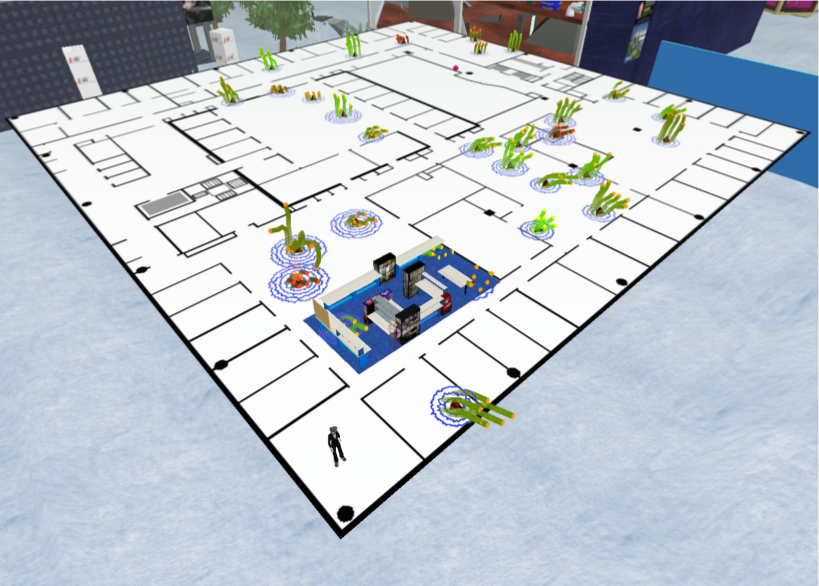
\includegraphics[width=\textwidth]{lifton_shadow_lab.png}
\caption{Side view of the final Shadow Lab structure, showing the two-dimensional floor plan of the third floor of the Wiesner building, three-dimensional reconstruction of the Media Lab, virtual data ponds and a human-sized avatar.}
\label{lifton_shadow_lab.png}
\end{figure}

\subsection{Ubiquitous Sensor Portals}

\textbf{This is getting closer to what this thesis is about, as we now have simultaneous visual interaction of both constituent environments, although only from pre-determined/fixed positions \& a more abstract virtual environment rather than the Shadow Lab of before (the stacked/time-travel image that has been removed from this document).}

Following on from the Dual Reality Lab, and now dropping the title dual reality in favour of cross reality, the Ubiquitous Sensor Portal project situated 45 I/O rich `portals', shown in figure \ref{ubiquitous_sensor_portal.jpg}, throughout the Media Lab, each with a corresponding extension in Second Life. Each portal comprised a myriad of environmental sensors (passive infrared (PIR) motion, light, sound, vibration, temperature and humidity) in addition to multimedia abilities via a camera, mounted on a motorised pan/tilt platform and capable of capturing still images as well as DVD-quality video, microphone and small touch screen display. They also featured active IR links that allowed them to communicate with various wearable badges in development by Media Lab researchers to identify users stood at a portal, and in addition could be used as reflection proximity sensors to detect the presence of unbadged users. When a user is present at a real portal, a white `ghost' is displayed by the corresponding virtual portal if they cannot be identified by badge, and their name displayed if they can. Video and audio from the real portal can be streamed into Second Life and a stream from a Second Life client streamed to the screen of the real portal.

\begin{figure}[h]
\centering
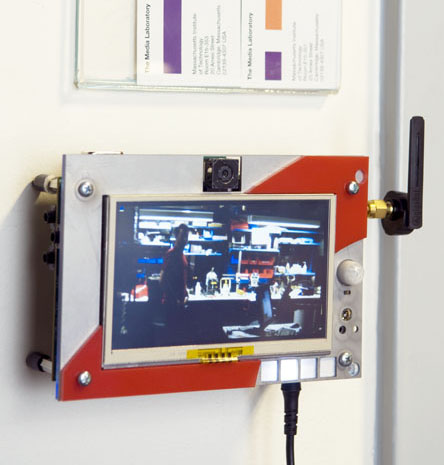
\includegraphics[width=0.6\textwidth]{ubiquitous_sensor_portal.jpg}
\caption{A Ubiquitous Sensor Portal.}
\label{ubiquitous_sensor_portal.jpg}
\end{figure}

However in stark contrast to the Dual Reality Lab, the virtual portals were not situated in a simulation of the real Media Lab in situations corresponding to their physical location, but instead used a more abstract virtual representation with a geometric layout; this design, shown in figure \ref{ubiquitous_sensor_portal_virtual.png}, reflected intellectual affiliation as opposed to real-world location and also allowed for intuitive browsing of past still images and videos captured by the real portal.

The ability of a person to walk about the real building and for their presence in front of different portals to be reflected in Second Life addressed the vacancy problem to some extent by allowing the user to explore the real environment in a normal fashion but for their position to occasionally be updated in the virtual environment. However the abstract layout of the virtual environment presents a method of virtual environments exploration disjoint to the physical layout and relationship between the portals themselves, which is not ideal for all applications.

\subsection{Doppellab}
\label{subsec:doppellab}

\textbf{This isn't really cross reality by anybody's definition \& is just a neat 3D visualisation of sensor network data.}

The current cross reality project undertaken by the Media Lab is the ongoing Doppellab, \textit{``an immersive, cross-reality virtual environment that serves as an active repository of the multimodal sensor data produced by a building and its' inhabitants''}~\cite{Dublon2011, Dublon2011a}. Doppellab uses the Unity3d game engine to allow users to visualise current and historic sensor data captured by a wide range of sensors distributed throughout the Media Lab in a three-dimensional virtual reconstruction.

However despite claiming to be a cross realtiy project, there is no evidence in the associated literature of any virtual-to-real, augmented virtuality data flow, which is a requirement of a cross reality system. Furthermore with regards to the vacancy problem, Doppellab \textit{``focuses on encouraging and enriching individual users' experiences of sensor data in 3-d environments''} and as such is of only passing interest to this review, as simultaneous presence in real and virtual environments must inherently support multiple users present in the same real and virtual surroundings to be of any great use.

\subsection{X-Reality}
\label{subsec:x-reality}
Marie Kim, Hwang Jae Gak and Cheol Sig Pyo at The Electronics and Telecommunications Research Institute, Korea, produced a Universal Sensor Network (USN) middleware, COSMOS, to address the issue of heterogeneity of sensor/actuator infrastructure that leads to difficulty in integrating them with virtual environments to establish a cross reality, or as they write it `X-reality', system~\cite{kim:practical}.

The matter of standards with relation to cross reality is discussed further in section \ref{subsec:sensor_actuator_infrastructure} however Kim et al.'s article is mentioned here as its introduction section frames and explains the cross reality paradigm well in terms of the principle features

\begin{quote}
\textit{``The important point of X-reality is a paradigm shift from single-directional information flows to bidirectional information flows between two worlds.''}
\end{quote}

and also how it can be employed for simultaneous presence in real and virtual environments

\begin{quote}
\textit{``The differential characteristic of X-reality is that it can augment user's engagement in the experiences of virtual presence and virtual world. Ultimately, it results in the human life span extension from the only real world to both worlds.''}
\end{quote}

\textbf{This quote is good for this thesis.}

\subsection{IEEE Pervasive Computing - Cross Reality Environments}
\label{subsec:ieee_pervasive_computing_-_cross_reality_environments}
The July-September 2009 issue of IEEE Pervasive (volume 8, number 3) was entitled `Cross Reality Environments' and serves both as attestation to the research promise of the paradigm and as a good survey of the state of the art in cross reality research at the time of publication. The issue is introduced by Roy Want~\cite{Want2009}, whose definitions and matrix representation of the different categories of alternate realities were discussed in section \ref{subsec:reality_matrix}, whilst the guest editor's introduction is provided by Joseph Paradiso, director of the Responsive Environments group at the MIT Media Lab~\cite{Paradiso2009}, whose work was discussed in section \ref{subsec:responsive_environments_at_mit_media_lab}.

Paradiso's introduction frames the background of cross reality very well, explaining the constituent technologies whose evolution will see the paradigm come to be, realising that it promises to serve as an extension of human perception and interaction and contrasting it with other alternate realities

\begin{quote}
\textit{We call the ubiquitous mixed reality environment that comes from the fusion of these two technologies cross-reality. Sensor networks can tunnel dense real-world information into virtual worlds, where this data is interpreted and displayed to dispersed users. Interaction of virtual participants can incarnate into the physical world through a plenitude of diverse displays and actuators. We can envision a user's interface into this environment as an extension of human perception and interaction, augmenting our five senses well beyond the canonical ``here and now'' and redefining the meaning of presence.''}
\end{quote}

Beth Coleman's article~\cite{Coleman2009} starts promisingly by further confirming that the terms cross reality and X-reality are interchangeable and then summarising the Eolus One project, an example application of cross reality, as further discussed in section \ref{subsec:eolus_one}.

Lifton and other members of the Media Lab also have an article in the issue~\cite{Lifton2009}, which primarily serves to summarise their current cross reality endeavours (including Plug, Shadow Lab, Ubiquitous Sensor Portals, Tricorder and Ubicorder), but also provides an interesting background to and future visions of the concept from their perspective, leading to this somewhat colourful quote

\begin{quote}
\textit{``We see cross-reality precipitating when diverse and ubiquitous sensor and actuator networks meet pervasively shared online virtual worlds, where phenomena freely tunnel between real and contrived continua at a multitude of ``wormholes'' opened by densely deployed networked devices, seamlessly adapting the level of immersion to match a variable ecology of available interfaces and user context or preference.''}
\end{quote}

\textbf{Gotta keep this `wormholes' quote...}

\subsection{Eolus One}
\label{subsec:eolus_one}
A project from Swiss construction, building services and real estate company Implenia, involving creative minds from SAP, Wago and Zumtobel, as well as some crossover with IBM, that ran for 2 years exploring concepts including building automation, energy monitoring, alert management and preventive maintenance~\cite{Coleman2009, UgoTrade2007}. Eolus One connected real-time data collection and distributed control mechanisms of smart buildings in the real world to a Virtual Command Center (VCC) hosted in Second Life. This connection was facilitated by a hardware and software platform that they created and dubbed the Virtual World Communication Interface (VWCI), which mediated communication between Second Life and various protocols in Building Automation Systems (BAS) including ZigBee, CANOpen and Modbus.

\subsection{IBM and Implenia}
In 2008, during the height of their investigation into virtual worlds, IBM announced their 3-D Data Center technology to allow the recreation of data centres in secure virtual worlds, bringing real-time data from different facilities into a 3D environment to visualize hot spots, data flow, server utilization and more to reduce cost, save time and help reduce carbon footprints~\cite{IBM2008, Marketwire2008}.
	
Implenia made use of these solutions to extend the functionality of their existing VCC (see section \ref{subsec:eolus_one}) by using IBM's virtual world integration middleware, Holographic Enterprise Interface (HEI), to add data from datacentre equipment to their existing virtual world models. Before the advent of this IBM technology Implenia's knowledge of the state of their data centres comprised only of information from the BAS and their VWCI, with no information from the servers themselves.

\begin{quotation}
	\textit{``Until working with IBM we only knew the state of our data center from the information we got through the building automation system and our virtual worlds communication interface. We didn't know the state of the server and information that was readily available to us until it was made more accessible via the 3-D visualizations that IBM built for us. We think that by combining this information with the information we had from the building automation side we can, from a building management standpoint, control the data much better and take action to be more efficient.''}~\cite{Marketwire2008}
\end{quotation}

\section{Position of Cross Reality}

\subsection{Position - \textit{Milgram \& Kishino}}
The position of XR in relation to other alternate realities studied by Computer Science can be visualised using Milgram \& Kishino's \textit{virtuality continuum} that stretches from an entirely real environment at one extreme to an ontologically parallel but entirely virtual environment~\cite{Qvortrup2002} at the other. The explanation herein distinguishes between environments themselves (depicted in figures \ref{virtuality-continuum-augmented-reality} to \ref{virtuality-continuum-cross-reality-3} by solid ellipses) \& where the stimuli that the user is perceiving originate from (depicted by dashed ellipses).

%Ontology - The core meaning within computer science is a model for describing the world that consists of a set of types, properties, and relationship types. There is also generally an expectation that the features of the model in an ontology should closely resemble the real world (related to the object).

Of particular importance is to appreciate the distinction between a XR system \& an \textit{augmented reality} (AR) system, as both concepts involve user engagement with both real \& virtual content. Whilst an AR system features a single environment, comprised of the user's RW overlain by some virtual content, with the user perceiving stimuli from this single augmented environment (figure \ref{virtuality-continuum-augmented-reality}), a XR system instead features two discrete environments, one real \& the other virtual, each complete unto itself (figure \ref{virtuality-continuum-cross-reality-1}).

Whilst AR falls within the realms of Mixed Reality (MR), a XR system can be considered as occupying the two extremes of the continuum outwith the MR region. However, XR systems that allow simultaneous interaction with both of their constituent environments blur this definition; using a XR platform such as that discussed in this document, a user can transition between perceiving stimuli from each of these environments (figures \ref{virtuality-continuum-cross-reality-2} \& \ref{virtuality-continuum-cross-reality-3}) in a manner that allows them to engage with each environment without becoming wholly vacant from the other.

\begin{figure}[h]
	\begin{center}
		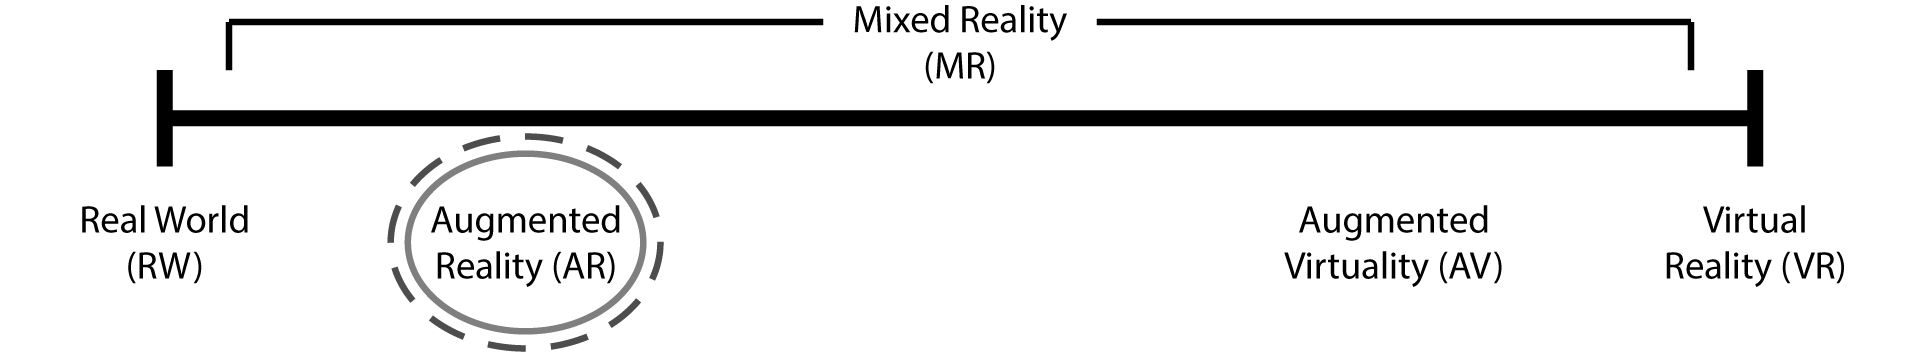
\includegraphics[width=\textwidth]{virtuality-continuum-augmented-reality.png}
		\caption{AR visualised using the virtuality continuum.}
		\label{virtuality-continuum-augmented-reality}
	\end{center}
\end{figure}

\begin{figure}[h]
	\begin{center}
		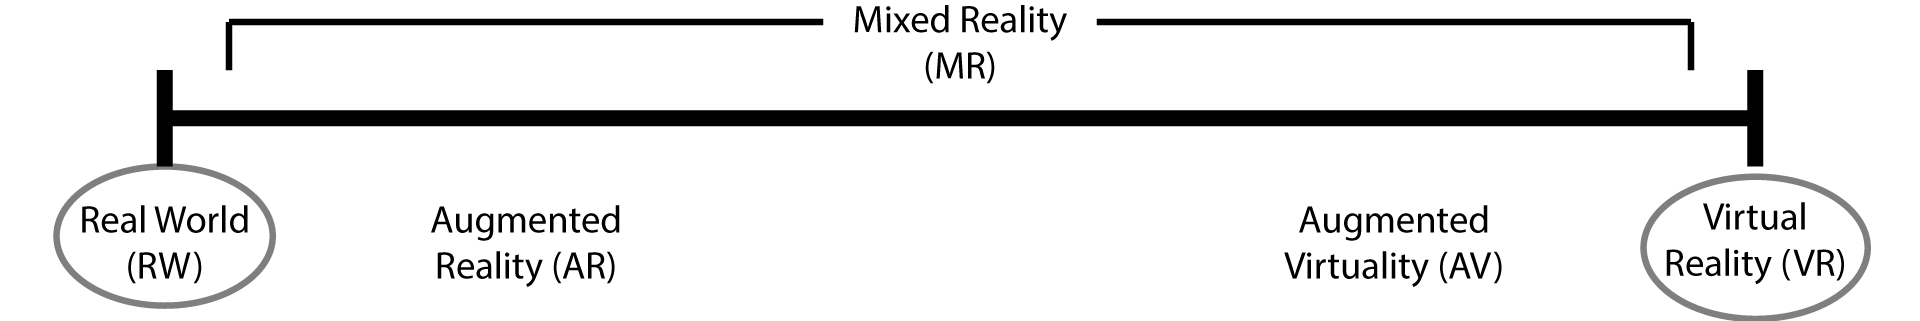
\includegraphics[width=\textwidth]{virtuality-continuum-cross-reality-1.png}
		\caption{The two environments that comprise a XR system.}
		\label{virtuality-continuum-cross-reality-1}
	\end{center}
\end{figure}

\textbf{Is it worth pointing out on the diagram that a true XR system would have a constant bi-directional stream of data between the two environments? And that without this, we have something like parallel reality?}

\begin{figure}[h]
	\begin{center}
		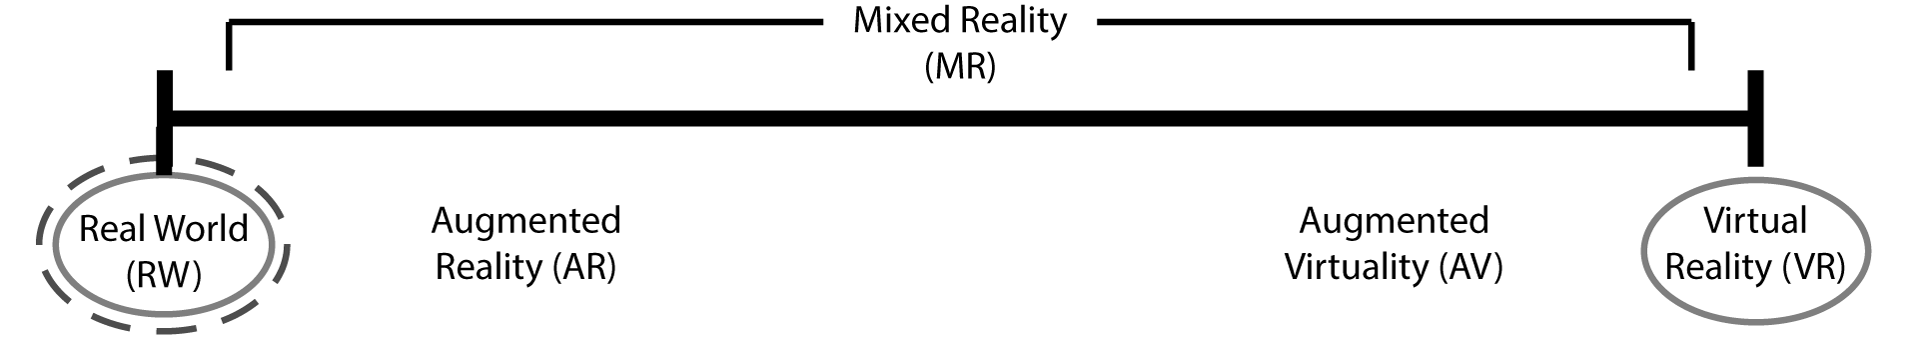
\includegraphics[width=\textwidth]{virtuality-continuum-cross-reality-2.png}
		\caption{A XR system with the user attending to RW stimuli.}
		\label{virtuality-continuum-cross-reality-2}
	\end{center}
\end{figure}

\begin{figure}[h]
	\begin{center}
		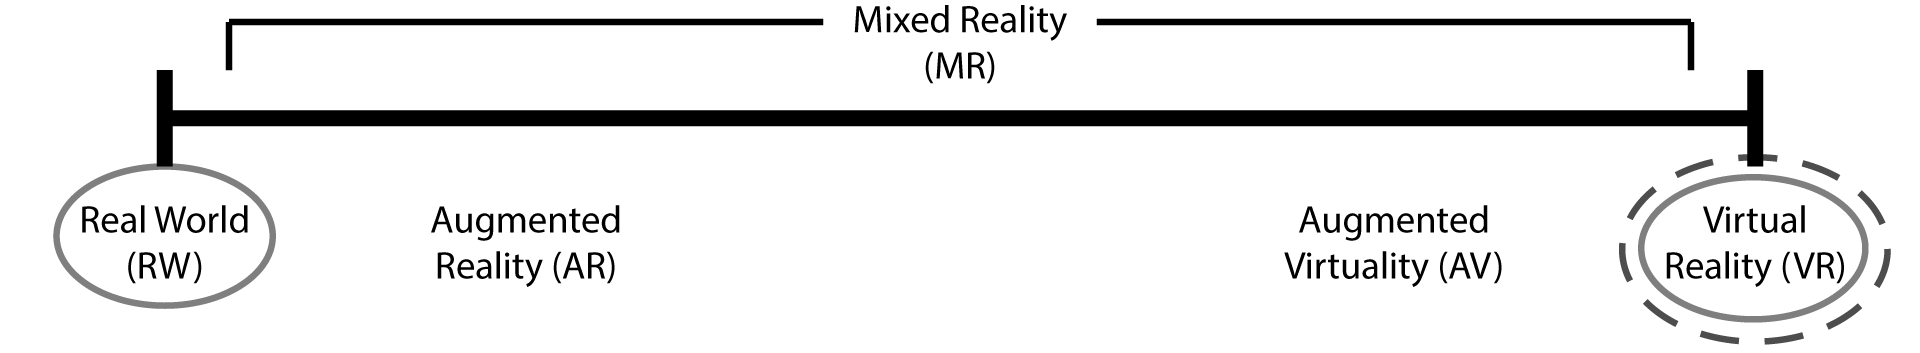
\includegraphics[width=\textwidth]{virtuality-continuum-cross-reality-3.png}
		\caption{A XR system with the user attending to VR stimuli.}
		\label{virtuality-continuum-cross-reality-3}
	\end{center}
\end{figure}

%=========================================================================================================

\begin{figure}[h]
	\begin{center}
		
\includegraphics[width=\textwidth]{virtuality-continuum-cross-reality-information-flows-dashed.png}
		\caption{The two environments that comprise a XR system, plus the bidirectional information flow between them.}
	\end{center}
\end{figure}

%=========================================================================================================

% More from experimental plan document

\section{Informing Mobile XR Implementation / On Presence}

\newcommand{\breakinpresencefootnote}{\footnote{The definition of \textbf{break in presence} adopted herein is the second from Waterworth \& Waterworth~\cite{Waterworth2001} (p205): a movement along the focus axis away from presence in the real or a virtual environment \& toward absence. This differs to Slater \& Steed's original definition in~\cite{Slater2000} as they considered presence only in terms of attending to stimuli from a virtual environment, with a break in presence as a Gestalt switch to instead attending to stimuli from the real environment. Waterworth \& Waterworth's model considers presence in terms of attending to stimuli from either the real \textit{or a virtual} environment, with a break in presence representing absence in the sense of heightened conceptual load \& the resultant reduced perceptual processing of environmental stimuli originating from \textit{either} the real or a virtual environment. This definition better fits the situation invoked by the Mirrorshades platform, which is concerned with intentionally \& willingly switching engagement between stimuli from both real \& virtual environments, rather than engaging with stimuli from only a virtual environment in a scenario where stimuli from the real environment are considered a `distraction'.}}

The novel aspect of the Mirrorshades platform is the ability it imparts upon its user to switch their locus of attention between equivalent vantage points in RW \& VR environments whilst walking around. This is achieved by the user performing transitions between RW visual stimuli \& VR visual stimuli, both presented via their HMD. This extends existing XR research by allowing the user to engage with the visual stimuli of the VR component of a XR system from any position \& at any time.

In order to achieve the highest quality of experience with this style of interaction with XR systems, it is vital to determine how best to implement these transitions; that is, to mitigate the increased cognitive load (manifesting as increased conceptual reasoning \& reduced perceptual processing, see section \ref{waterworth}) required to comprehend these transitions, as this increased cognitive load will detract from engagement with the environments \& reduce the user's willingness to perform these transitions.

Whilst some researchers support the notion that in systems where more than one environment competes for the user's locus of attention there is an `all or nothing' Gestalt switch between awareness of one environment \& the other~\cite{Slater2002}, which would result in a substantial increase in cognitive load upon each transition, Mirrorshades has been developed in support of the contrary opinion; that switching locus of attention from the stimuli of one environment to those of another does not completely overrule the user's awareness of the former, that both environments can be perceived at the same time (albeit one to a lesser extent)~\cite{Ijsselsteijn2001} \& that when engaging with VR content a user's focus can even be said to typically be \textit{shared} between VR \& RW~\cite{Waterworth2001}.

This latter position is particularly apt for situations wherein the RW \& VR environments share the same fundamental layout \& dimensions, as those in a XR system often do, as the inherent familiarity between the two environments reduces the cognitive load associated with transitioning between them. Furthermore, the notion of experience of presence as changing continually from moment-to-moment~\cite{Heeter2003, Ijsselsteijn1998} lends confidence to the successful mitigation of the cognitive load associated with these transitions to manageable levels. One might even liken this `switching' between RW \& VR to the `cycling through' behaviour observed in users of virtual communities, which stemmed from the `window' concept of modern computer operating systems~\cite{Turkle2004}.

However, no matter how smooth the transition the process is expected to always result in some heightened cognitive load, a temporary \textit{break in presence}\breakinpresencefootnote{} (BIP), as the user comes to terms with the new environment presented to them \& comprehends its relation to the other environment that they were just perceiving.

%\section{Transitions}
Transitions can be performed in multiple different manners \& it is hypothesized that users will prefer different styles of transition in different situations, surroundings \& scenarios (where `preference' toward a particular style of transition is expected to correlate strongly with a less severe BIP being experienced upon its execution).

To this end, several different transition methods have been developed \& this investigation will endeavour to identify \& quantify preferences toward them, to infer which approaches to transitioning between RW \& VR visual stimuli are more or less appropriate for the different situations that arise where a platform like Mirrorshades may be deployed. In particular, it is hypothesized that there will be a strong correlation between participant movement (or lack thereof) \& choice of particular transition style.

\subsection{Transitions using the Combined Model}
Visualised using the combined model (see section \ref{waterworth}) as figure \ref{focus-locus-sensus-with-virtuality-continuum-with-transition}, these transitions are an oscillation along the locus axis, between a RW environment at one position \& a VR environment at the other.

Heightened cognitive load required to comprehend a transition is a temporary movement upon the focus axis from presence toward absence (a BIP). With the ability of a wide FOV, stereoscopic 3D, head-tracked HMD to produce immersive VR visual stimuli that require fairly limited cognitive processing \& our inherent ability to engage with our RW surroundings without significant cognitive load, focus is expected to be high (toward the presence extremum) when attending to stimuli from either RW or VR.

Sensus is expected to be largely task dependent, however when performing a task that involves actively engaging with the visual stimuli from either/both of RW or VR it is expected to be high (toward the conscious extremum). Upon triggering a transition, sensus is expected to increase, as the user centres their attention upon relating the visual stimuli from the new environment to those they were just perceiving from the other environment

%Whilst continued exposure to the platform is expected to reduce the severity of the BIPs, mitigating their severity from the outset (reducing the displacement from the presence extremum downwards toward absence) through informed execution of the transitions between RW \& VR is believed to be important to the overall quality of experience that users receive.

%absent-mindedness - caused by increased attention toward a single object of focus (hyperfocus, eg the object of focus is the switch)
% or caused by distraction (again, the switch)

%\clearpage

%\vspace{12mm}

%\begin{figure}[h]
%	\begin{center}
%		
\includegraphics[width=0.7\textwidth]{images/focus-locus-sensus-with-virtuality-continuum-with-transition.png}
%		\caption{Operation of the Mirrorshades platform represented upon the combined model.}
%		\label{focus-locus-sensus-with-virtuality-continuum-with-transition}
%	\end{center}	
%\end{figure}

\begin{figure}[h]
	\begin{center}
		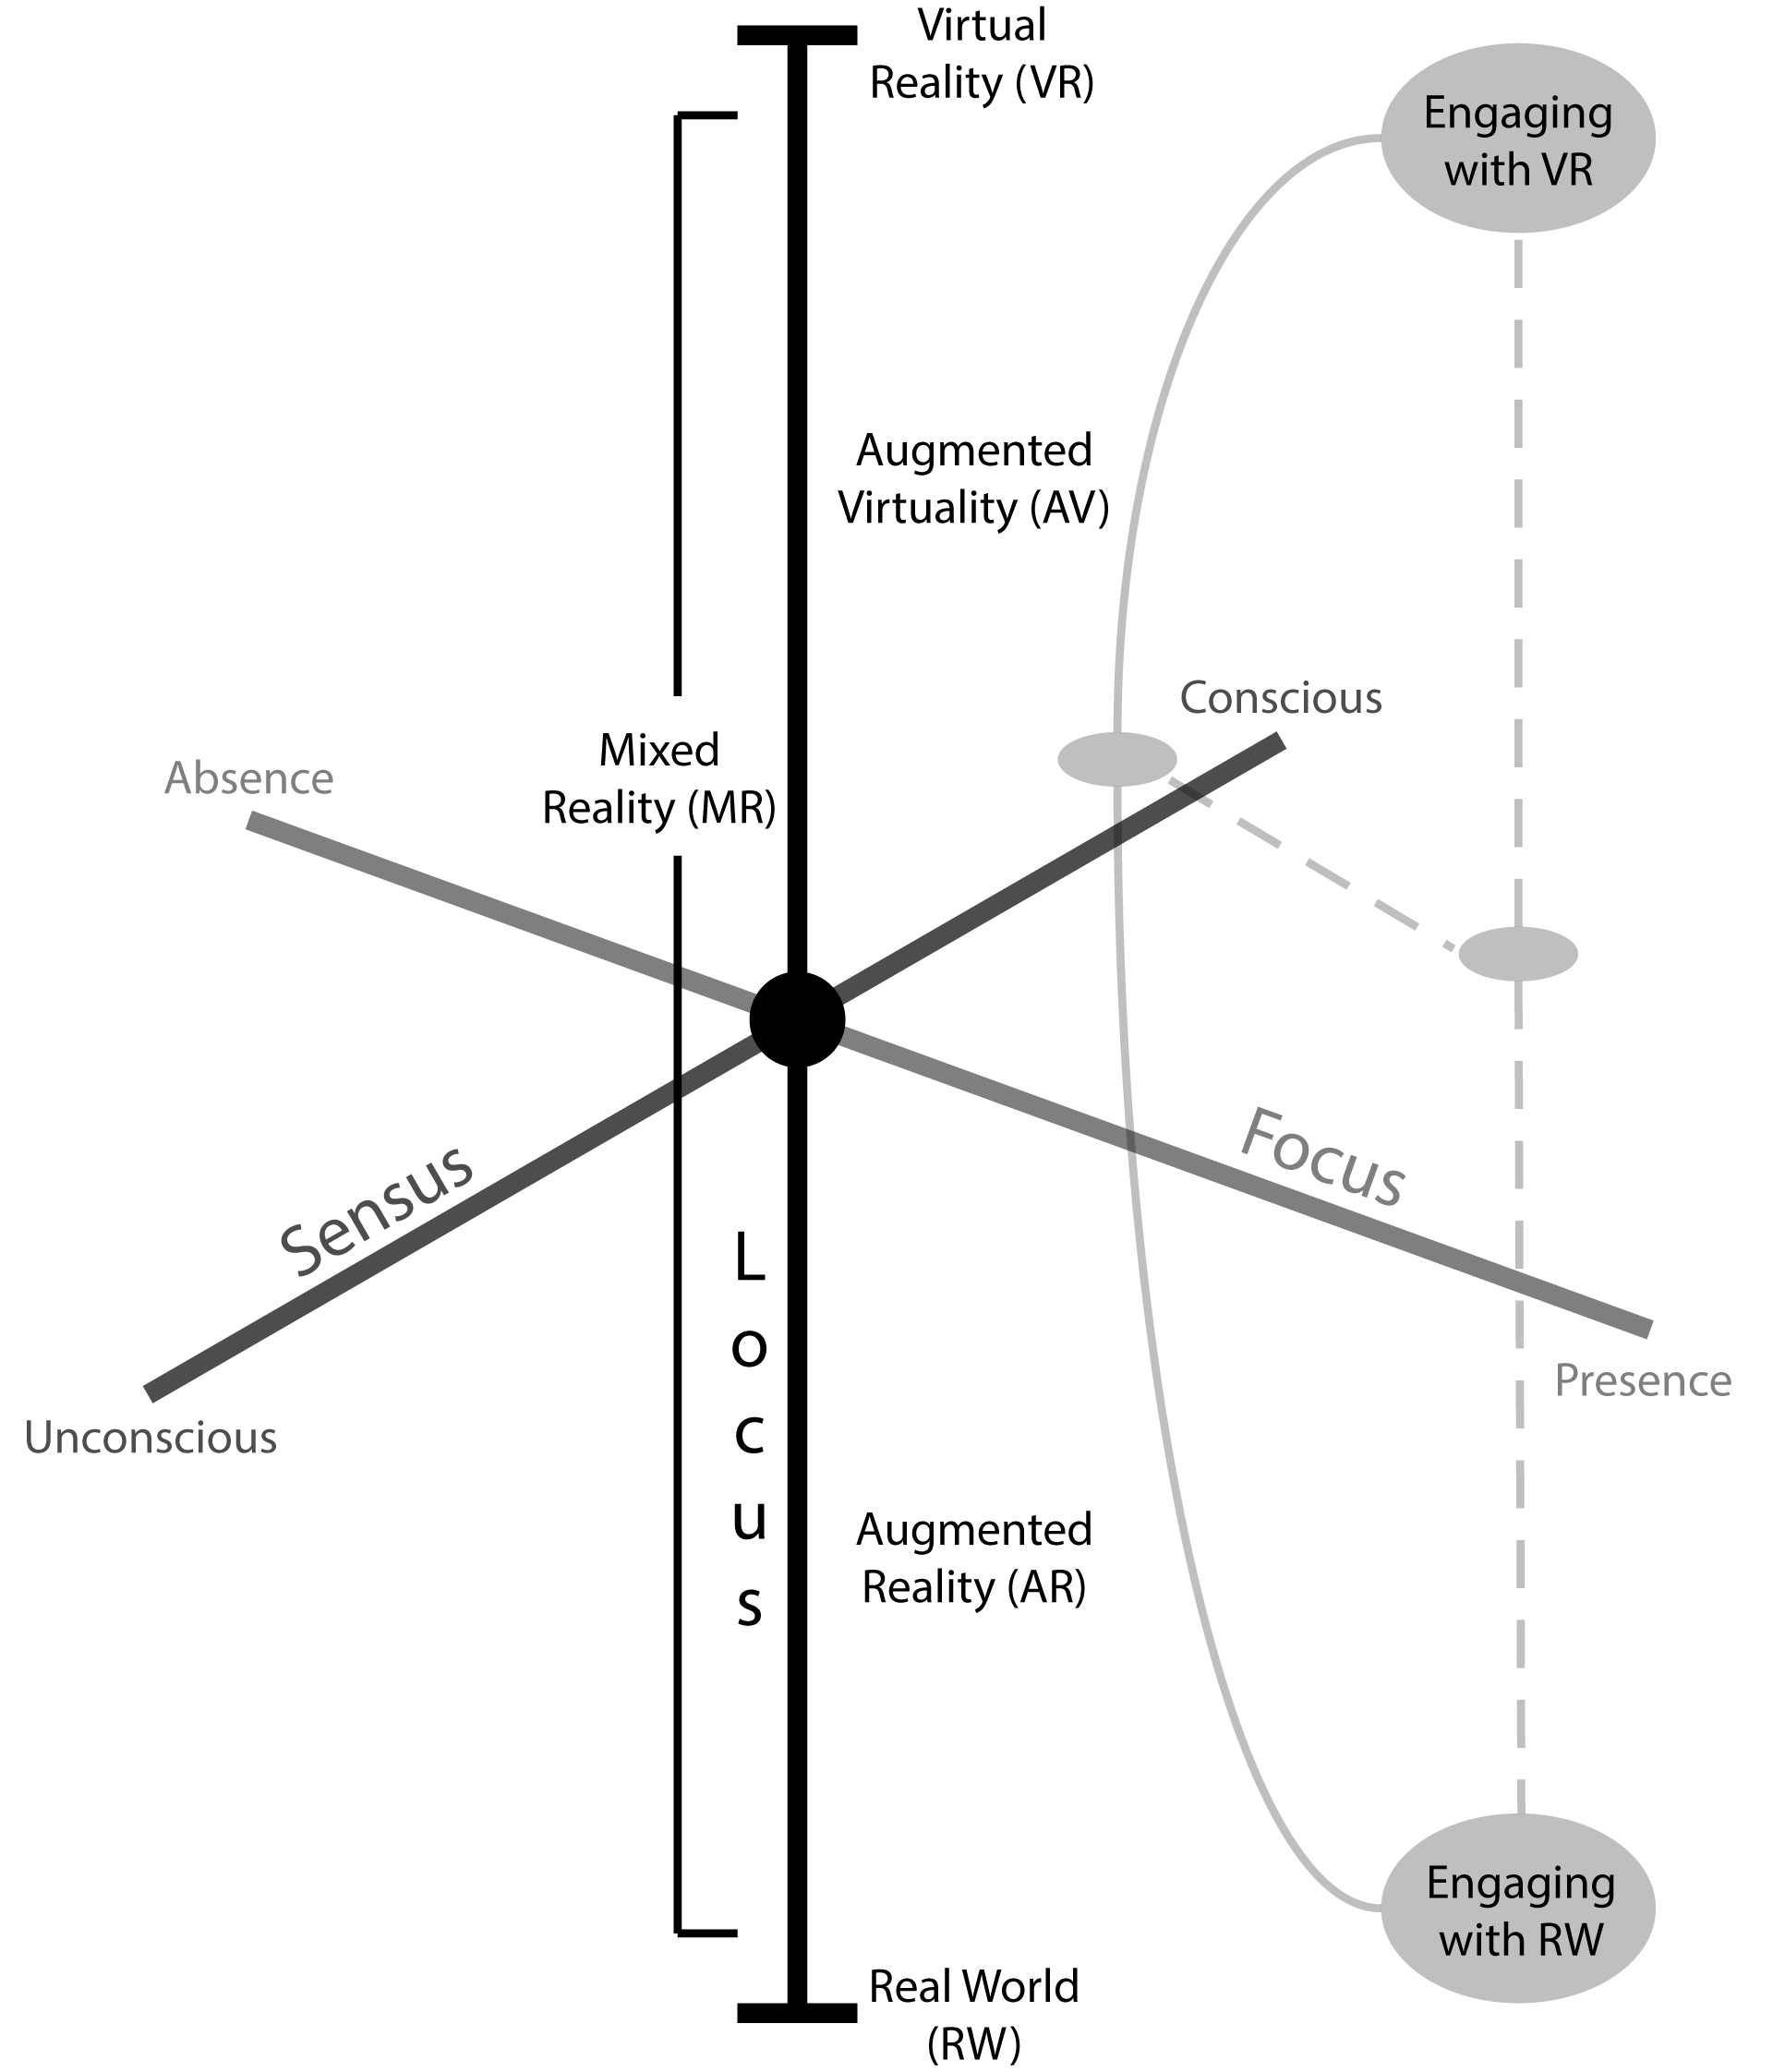
\includegraphics[width=0.7\textwidth]{focus-locus-sensus-with-virtuality-continuum-with-transition-updated.png}
		\caption{Operation of the Mirrorshades platform represented upon the combined model.}
		\label{focus-locus-sensus-with-virtuality-continuum-with-transition}
	\end{center}	
\end{figure}

%=========================================================================================================
%=========================================================================================================

% Original literature review from here on

Reviewing the literature on the domain of alternate realities this research finds that there is a gap in the scholarly investigation of simultaneous presence in real and virtual environments and the associated `vacancy problem'. This review proposes that a better understanding of the extension of human presence from only one of the real world or a virtual environment to simultaneous presence in both will permit the introduction of novel systems in a variety of fields in which simultaneous interaction and exploration of both real and virtual environments is possible. Such systems will likely be formed by expansion of research into \textit{cross reality}, an alternate reality comprised of complete real and virtual environments able to mutually reflect and influence each other via sensor/actuator infrastructure, and are likely to be in high demand as progress toward 3D extension of the Web continues.

\section{Conclusions}
We are rapidly approaching a situation in which ubiquitous sensor/actuator infrastructure allows us to access vast amounts of information about any location at any time and additionally to act upon this information and affect these locations. The continuing adoption of fast Internet connections, the increasing ability of commodity hardware including portable devices such as mobile phones and tablets to render complex three-dimensional graphics, and the development of 3D multi-user virtual environments that place an emphasis on notions of community, creation and commerce instead of competitive gaming, all point toward a continuing natural progression toward 3D extension of the Web on a large scale.

It is already common to see people spending substantial amounts of time immersed in the 2D textual/graphical Web whilst simultaneously interacting with the real world around them. This desire to maintain a Web presence whilst simultaneously interacting with the real world is set to remain as interaction with the Web evolves from 2D to 3D. Thus it is prudent to investigate approaches for implementing and applications for exploiting the concept of simultaneous presence in real and virtual 3D environments, whether spatially equivalent or not.

This review has unearthed a plenitude of research on numerous alternate realities, either experienced in isolation from other realities (reality, virtual reality) or by mixing limited amounts of one with another (augmented reality, augmented virtuality) however has discovered a comparative lack of research attention focussed on the concept of simultaneous presence and interaction with two complete environments, one real and the other virtual. Cross reality is the closest existing concept, however the vast majority of the research in this field has used statically located computers to access the virtual environments, preventing users from exploring or interacting with the real environment that is not immediately surrounding them; the true notion of simultaneous presence in real and virtual environments requires freedom of movement and interaction with both environments, perhaps by adopting a manner of interaction with the virtual environment similar to that of the VTW project.

This deficiency of research into simultaneous presence in real and virtual environments warrants addressing with further academic investigation, as it represents a style of interaction that is bound to become commonplace as progress toward 3D extension of the Web continues at an accelerated pace.
